% coding:utf-8

\section{Digitally-Controlled Oscillator}

\subsection{Übersicht}
\begin{frame}
  \begin{center}
\tikzstyle{block} = [ draw,fill=blue!20,text width=5em,align=center,
                      rounded corners,minimum height=3em]
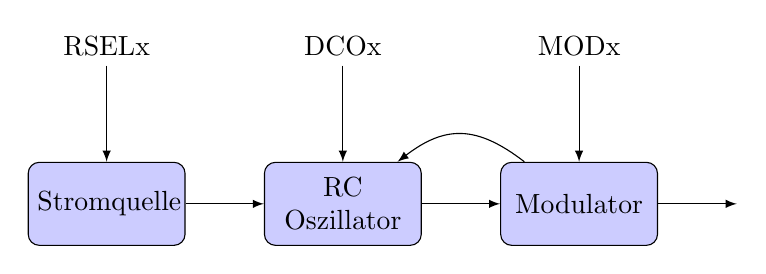
\begin{tikzpicture}
  \uncover<1->{\node[block] at (0,0) (iq) {Stromquelle};}
  \uncover<2->{\node[block] at (3,0) (osc) {RC Oszillator};}
  \uncover<3->{\node[block] at (6,0) (mod)   {Modulator};}
  \uncover<4->{\node at (0,2) (rselx)   {RSELx};}
  \uncover<5->{\node at (3,2) (dcox)   {DCOx};}
  \uncover<6->{\node at (6,2) (modx)   {MODx};}
  \uncover<1->{\draw[-latex] (iq.east) -- (osc.west);}
  \uncover<2->{\draw[-latex] (osc.east) -- (mod.west);}
  \uncover<3->{\draw[-latex] (mod.east) -- ++(right:1);}
  \uncover<4->{\draw[-latex] (rselx.south) -- (iq.north);}
  \uncover<5->{\draw[-latex] (dcox.south) -- (osc.north);}
  \uncover<6->{\draw[-latex] (modx.south) -- (mod.north);}
  \uncover<6->{\draw[-latex] (mod) .. controls (4.7,1) and (4.3,1) .. (osc);}
\end{tikzpicture}
\end{center}

\end{frame}

\subsection{Modulation}
\begin{frame}
  \begin{tikztimingtable}
    \mbox{\uncover<1->{MOD =  0}} & <1->33L<*>\\
    \mbox{\uncover<2->{MOD =  1}} & <2->16LH16L<*>\\
    \mbox{\uncover<3->{MOD =  2}} & <3->8LH15LH8L<*>\\
    \mbox{\uncover<3->{MOD =  3}} & <3->8L2{H7L}H8L<*>\\
    \mbox{\uncover<4->{MOD = 16}} & <4->L16{HL}<*>\\
    \mbox{\uncover<4->{MOD = 24}} & <4->L8{3HL}<*>\\
    \mbox{\uncover<4->{MOD = 31}} & <4->L31HL<*>\\
  \end{tikztimingtable}
\end{frame}

\subsection{Kalibrierung}
\begin{frame}
  \begin{figure}
    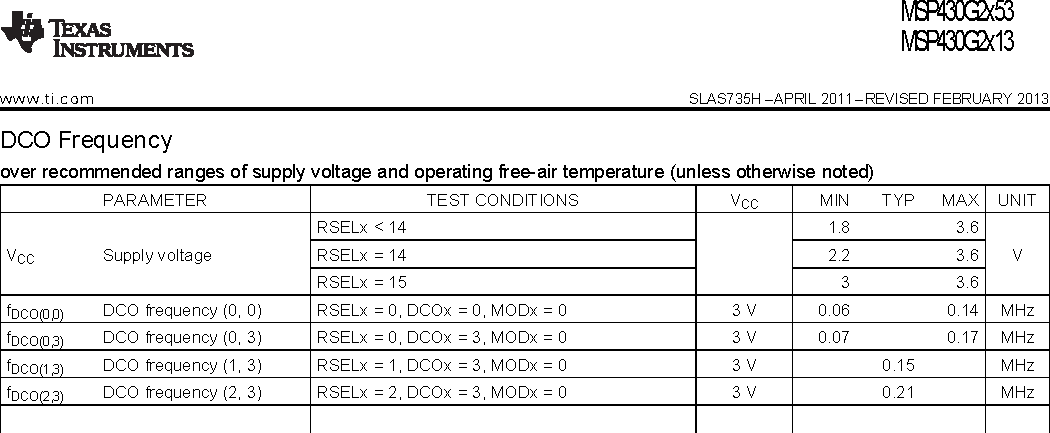
\includegraphics[width=1.0\columnwidth]{fig/ti_ds_dco_freq.pdf}
    \caption{Auszug aus dem Datenblatt des MSP430G2553}
  \end{figure}
\end{frame}
\begin{frame}
  \begin{itemize}
    \item Texas Instruments \pause \\
      MSP430F2x $\rightarrow \pm 1 \%$ \pause \\
    \item Inbetriebnahme \pause
    \item FLL
  \end{itemize}
\end{frame}